\section{Fixed removal}



In the pursuit of modelling multi-stage intracellular infection, we have been working on an iterated birth death catastrophe process with the assumption of complete transfer (chained ruptures). In trying to determine whether there is a fundamental reason for bursting dynamics in pathogenesis, this model is of limited efficacy. With agents replicating identically whenever they are within a host cell, it matters not how they are moved, just that they are replicating. With chained ruptures, the burst event is merely a recorded instance without tangible implication to agent spread. And if instead, the bacteria modelled were to make their way one by one to a new host, or even to multiple hosts, no change would be made to the expected growth rate of the overall population. Even if some delay were introduced for unit transfer between hosts, this would merely have the effect of adding intervals of inactivity to the time axis; broad propagation dynamics would remain identical.\par

It seems that if we wish to begin understanding why, or if there is a reason why, pathogens follow a bursting regime of infection, we must consider additional factors. Namely, we must take into account that the death and replication rates of individual agents are not entirely independent to the surrounding cohort. For example, various of the bodies immuno-factors are depletable. For instance, leucocytes including macrophages and neutrophils contain on the order of 10 so called granules. Small packets containing oxidising compounds with a toxic effect on invading pathogens. Given these can be used up, the effective within-host death rate of infectious agent will reduce as more and more of the incident cohort are killed. There are likely extracellular immune factors which exhibit a similar pattern of depletion.\par

Here is presented an extension to the ``chained rupture'' model. There is included a simple assumption which arises from an argument of immuno-depletion: that following a burst release event, some defined fixed count of the agents are removed. This is used as the basis for attempting to understand whether bursting pathogenesis strategies might be of fundamental advantage in relevant cases.


\subsection{Successive birth death catastrophe}
\noindent
The concept of chained ruptures is simple. A series of BDC processes follow on from one another, the result of the last going on to found an initial condition for the next.\par
Starting with an single replicative unit, the first process undergoes the standard dynamics of birth and death. Then, at the time of the catastrophe event, the quantity of units present is, as it were, immediately transfers into another target cell founding the second process with its initial condition as given. This is the main assumption: that released replicative units somehow find their way, all at once, to the same host cell. Of course this is quite reduced from the biological context.\par
A less restricted view would be that following rupture, all of the $r_1$ released bacteria undergo Brownian motion and drift gradually from the burst location. The cohort, as it spreads out will encounter multiple new target cells and get taken up one by one. Albeit less so, this is also greatly reduced from biological reality, which in its full complexity will be beyond the scope of concise mathematical description. For example, the target cells we have focused on mostly are macrophages. Macrophages do not merely float around in Brownian drift; they are motile, and essentially walk around their environment seeking out debris and alien material to engulf and make away with. The agents themselves are little more straightforward. Yersinia pestis can ``decide'' whether it will be absorbed or not by such phagocytes. In addition to this, the bacteria can inject immune cells with a host of special proteins with various effects including neutralisation.\par
Generally, the playing field of these actors is just that, an environment of play, in which the responsive agents interact with one another; causal relationships ensue which go far beyond mere drift and chance.\par

\subsection{Extracellular removal}



\begin{figure}[H]
    \centering
    % First figure
    \begin{subfigure}{0.31\textwidth}
        \centering
        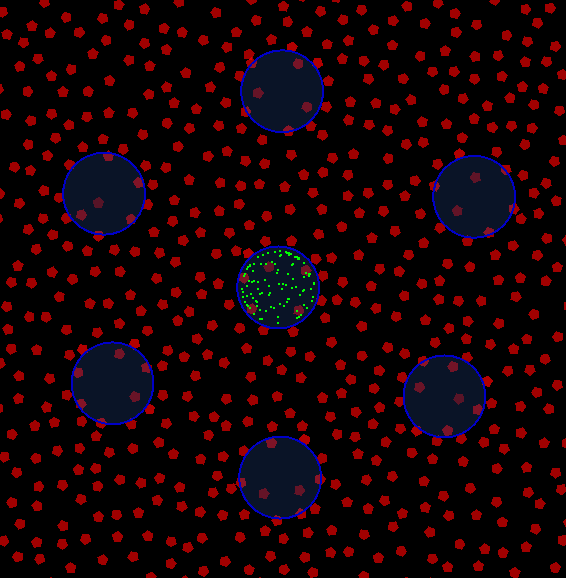
\includegraphics[width=\textwidth]{figures/IMG_ch7/Bursting/FR/big1} % Adjust the image path as necessary

        \label{fig:figure1}
    \end{subfigure}
    \hspace{\fill} % Optional: adds space between figures
    % Second figure
    \begin{subfigure}{0.31\textwidth}
        \centering
        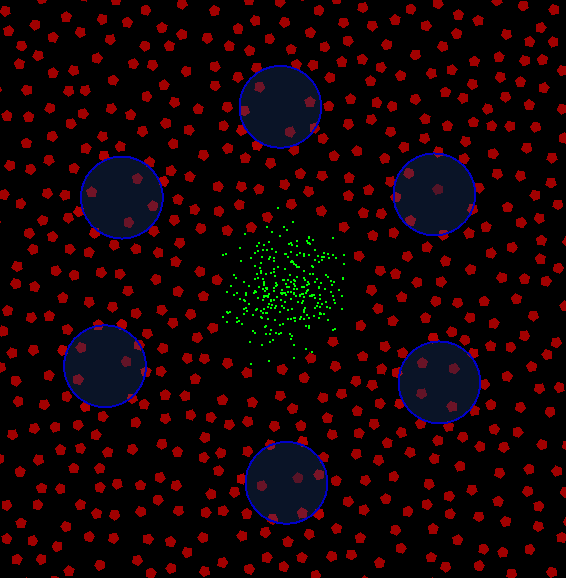
\includegraphics[width=\textwidth]{figures/IMG_ch7/Bursting/FR/big2} % Adjust the image path as necessary
    
        \label{fig:figure2}
    \end{subfigure}
    \hspace{\fill} % Optional: adds space between figures
    % Third figure
    \begin{subfigure}{0.31\textwidth}
        \centering
        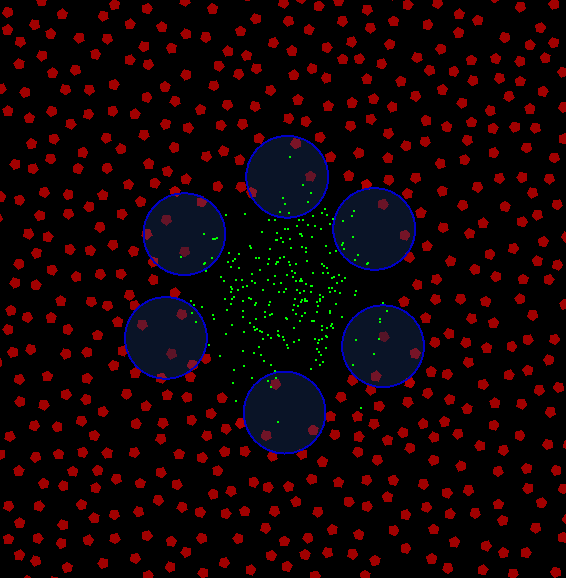
\includegraphics[width=\textwidth]{figures/IMG_ch7/Bursting/FR/big3} % Adjust the image path as necessary
    
        \label{fig:figure3}
    \end{subfigure}

    \caption{In the above simlation run snapshots, it is demonstrated that given the presence of depletable extracellular immuno factors, a larger released pathogenic load creates a safety in numbers "flooding effect" leading to more incident pathogen in surrounding host cells.}
    \label{fig:three_figures}
\end{figure}



\begin{figure}[H]
    \centering
    % First figure
    \begin{subfigure}{0.31\textwidth}
        \centering
        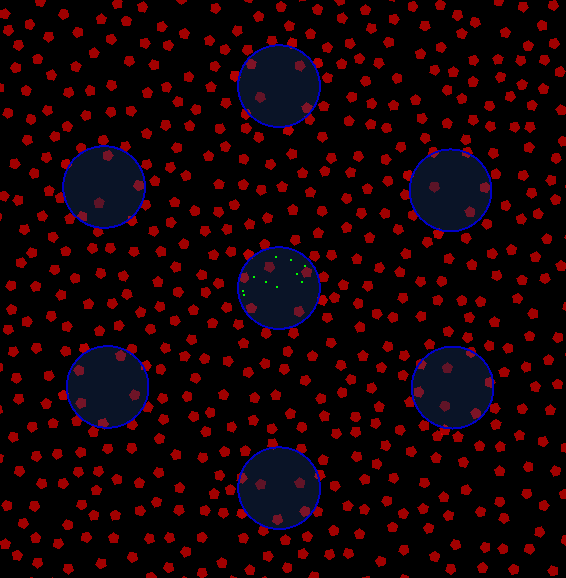
\includegraphics[width=\textwidth]{figures/IMG_ch7/Bursting/FR/small1} % Adjust the image path as necessary
        \label{fig:figure1}
    \end{subfigure}
    \hspace{\fill} % Optional: adds space between figures
    % Second figure
    \begin{subfigure}{0.31\textwidth}
        \centering
        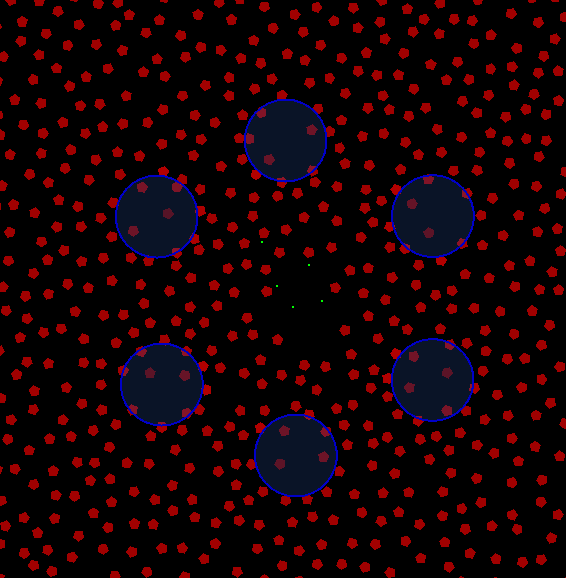
\includegraphics[width=\textwidth]{figures/IMG_ch7/Bursting/FR/small2} % Adjust the image path as necessary
        \label{fig:figure2}
    \end{subfigure}
    \hspace{\fill} % Optional: adds space between figures
    % Third figure
    \begin{subfigure}{0.31\textwidth}
        \centering
        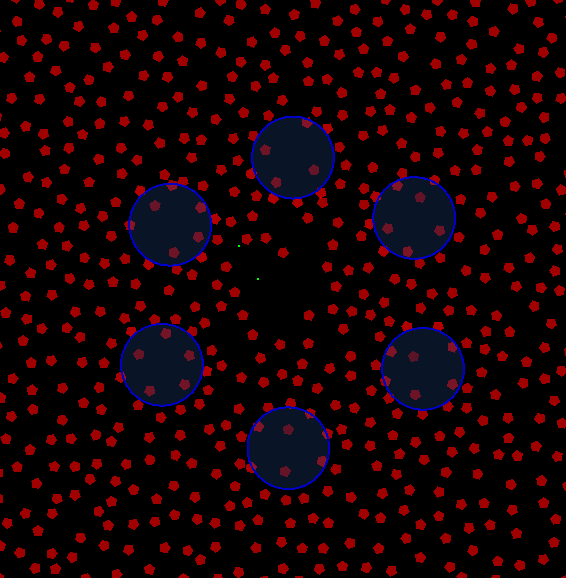
\includegraphics[width=\textwidth]{figures/IMG_ch7/Bursting/FR/small3} % Adjust the image path as necessary
        \label{fig:figure3}
    \end{subfigure}

    \caption{Contrasting the above situation, a small released load may be depleted without persistence to the next rounds of intracellular absorption and replication.}
    \label{fig:three_figures}
\end{figure}




\subsubsection{The assumption}
But let us humour it --- this concept of spatial drift. Despite imperfection, it does improve on the simpler dynamic of chained immediate transfer. Picture the playing field: a three dimensional extracellular matrix populated by three types of agents: replicative units (pathogen), Host cells (Macrophages), and another type of immuno-active cell; we'll call them simply ``killer cells''. This third type is able to eliminate the units of pathogen on contact, being used up in the process; one to one encounters where a killer cell removes a replicative agent and itself from play.\par
To begin with, the extracellular matrix is populated evenly with target cells and killer cells, each group occupying the space in a uniform spatial density. Killer cells are smaller and more numerous than target cells; a greater number per unit volume. Dynamics within target cells are as we understand in the birth death catastrophe process. The units of pathogen replicate and die within the cell until eventually rupture is caused and the load is released.
In this model, we are considering movement to be Brownian. An extracellular colony will drift from their burst location, spreading out and coming into contact with surrounding cells. Some will encounter target cells, others, killer cells. Now... my intention with this is not to construct a full mathematical description of this model game. This would be cumbersome and intractable. It will be possible to simulate it computationally, and this may prove helpful in supporting the assumption which I hope to use the model to justify. If we suppose that no new killer cells are introduced into the environment. An assumption that pathogen movement and absorption occurs on a shorter time scale thank killer generation. Then, with greater burst sizes, each individual bacteria will have a smaller probability of being removed. Those at the leading edge, as it were, clearing the way for their comrades in the rear.

If it happens that free agents do tend to find a new host before long --- an assumption taken to the limit in the case of chained immediate transfer --- this above observation offers the basis of an approximate mathematical rule. That is, there will be a relationship between burst size and the number of pathogen killed in the process of transfer. 

As bursts of greater and greater number are compared, the casualty count will increase more and more slowly. Qualitatively this might be like a logarithmic progression.

$$\theta(r) \sim \log(r+1),$$  
where $r$ is a given burst size and $\theta$ is the number of replicative agents removed by killer cells. (The +1 is simply to make the curve go through the origin).



\begin{figure}[H]
\begin{center}

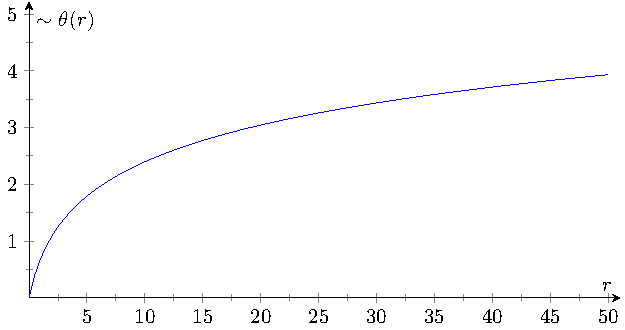
\includegraphics[width = 0.7\textwidth]{figures/IMG_ch7/log_plot1.pdf}

\end{center}
\caption{Qualitative representation of the deminishing removed count $\theta(r)$, given released numbers.}
\end{figure}
    

\noindent
Given this to be the case, it might prove reasonable to impose a fixed removal following release. In this construction, the number removed by killer cells will be a specified constant, regardless of burst size. Though, if the burst size is less than this constant, simply all of the units will be killed. 
$$\text{removal} = \begin{cases}
& r , \quad \text{ if }r \leq \theta\\
& \theta, \quad \text{ if } r>\theta.
\end{cases}$$
Now taking $\theta$ to be a constant.

	
\begin{figure}[H]
\begin{center}

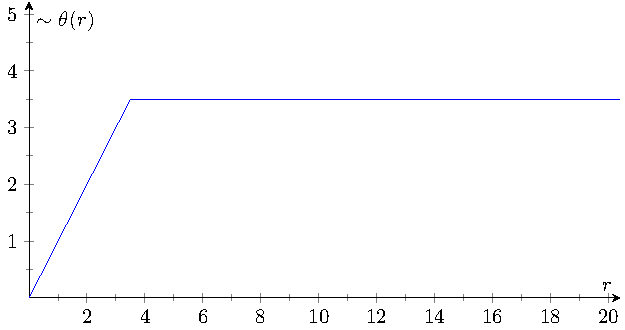
\includegraphics[width = 0.7\textwidth]{figures/IMG_ch7/log_plot_square.pdf}

\end{center}
\caption{An approximate representation of the above shown (figure above) diminishing removel effect.  Fixed removal count $\theta$ facilitates analysis of proliferation number.  (the number of new infections provided by a single burst event assuming one pathogen per new host.)}
\end{figure}

    
    
    


\noindent
The potential efficacy of this assumption rests in the likelihood that the same qualitative dynamics will be shared with the case of logarithmic removal (or whatever the actual relation is, assuming it is of this sort). 

There are a couple of points to address.
\begin{itemize}
\item I want to impose a further assumption: that at the time of each rupture event, the killer cell prevalence has returned to it's steady state and is once again of uniform spatial distribution.

\item We may frame the ``fixed removal'' dynamic in the context of chained transfers where all agents released have the same target cell to go to. Or, we may consider a case in which each successful pathogenic unit goes on to found an infection in a new target cell. 
\end{itemize}

\vspace{10pt}


\hrule
\vspace{5pt}

\noindent
\textbf{Aside:} In the case where all surviving agents go directly to the same host cell, we can potentially frame the replication ratio as follows: Expected number of surviving released units \textit{per incident agent}. 
\hrule
\vspace{8pt}


\vspace{10pt}


\noindent
Let us for now take this second option --- that each released cell goes on to found a new infection in a new target cell. We can consider the effective replication number between target cell infections. That is, the expected number of newly infected target cells created by a given host of one initial bacterium. Because each surviving released infectious particle infects a new host, the replication number is simply the expected quantity of these survivors. 

\subsubsection{Intra-burst replication ratio}
To begin with, we must define $r$: the outcome of a BDC process with a single incident unit. Mainly, we much choose, whether or not to include outcomes that are 0 due to process death. It makes practical sense for our purpose to choose this option, to not ignore cases of $r = 0$. With this $\mean{r} = \lim_{t\to\infty} \mean{\yt} = V_{\text{inf}}$.\par

The number that survive our fixed removal will be $\max({0, r-\theta})$. Hence, the expected replication number is
$$R_0 = \mean{\max(r-\theta, 0)}.$$
We can deconstruct this based on whether the burst size is bigger or smaller than $\theta$:
\begin{align*}
\mean{\max(0, r-\theta)}  &= \mean{r-\theta | r \geq \theta} \pr{r\geq \theta} + \cancelto{0}{ \mean{0}\pr{r<\theta}}\\
& = \lrbs{\mean{r| r\geq \theta} - \theta}\pr{r\geq\theta}
\end{align*}
Then, we can extract $\mean{r|r\geq\theta}$ in the following way. 
$$\mean{r} = V_{\text{inf}}= \mean{r|r\geq\theta}\pr{r\geq 0 }  + \mean{r | r < \theta }\pr{r < \theta}$$
With 
$$\pr{r<\theta} = \sum^{\theta - 1}_{i=0} \pr{r = i},$$
$$\pr{r\geq \theta} = 1- \pr{r<\theta} ,$$
and,
$$\mean{r|r<\theta} = \sum^{\theta - 1}_{i=1} i \pr{r = i| r < \theta} =  \sum^{\theta - 1}_{i=1} i \frac{\pr{r = i}}{\pr{r < \theta}},$$
we can make the rearrangement,
\begin{align*}
\mean{r|r\geq\theta} &= \frac{\mean{r} - \mean{r|r<\theta} \pr{r<\theta} }{\pr{r\geq \theta} }\\
&= \frac{\mean{r} -       \sum^{\theta - 1}_{i=1} i \frac{\pr{r = i}}{\cancel{\pr{r < \theta}}}  \cancel{\pr{r<\theta}} }{\pr{r\geq \theta} }\\
&= \frac{\mean{r}  -   \sum^{\theta - 1}_{i=1} i \pr{r = i} }{1 -  \sum^{\theta - 1}_{i=0} \pr{r = i}}.
\end{align*}
This is analytically computable because we have 
$$\pr{r=i} = \frac{\delta}{\lambda}\lrb{\frac{1}{a}}^i$$
$$\mean{r} = V_{\text{inf}}. $$
Hence,
$$\mean{\max(0,r-\theta)}  =  \lrbs{  \frac{\mean{r}  -   \sum^{\theta - 1}_{i=1} i \pr{r = i}}{1 -  \sum^{\theta - 1}_{i=0} \pr{r = i}}   - \theta} \pr{r\geq \theta}  $$
becoming 
$$\mean{\max(0,r-\theta)}  =  \lrbs{ \frac{V_{\text{inf}} -  \mathcal{K} }{1 -  \mathcal{G}} - \theta} \lrb{1 - \mathcal{G}}  = V_{\text{inf} }-  \mathcal{K} - \theta ( 1 -  \mathcal{G})$$
where 
$$\mathcal{G} = b+ \sum^{\theta - 1}_{i=1} \frac{\delta}{\lambda}\lrb{\frac{1}{a}}^i   \quad\text{ and } \quad \mathcal{K} =  \sum^{\theta - 1}_{i=1} i  \frac{\delta}{\lambda}\lrb{\frac{1}{a}}^i . $$
Because the formula 
$$\pr{r=i} =  \frac{\delta}{\lambda}\lrb{\frac{1}{a}}^i$$ does not correctly apply when $i = 0$, this is why the sum for $\mathcal{G}$ begins at 1, and why there is the term, $b$, preceding the sum. This is the probability that the process ultimately ends in death, an output of 0. 


\vspace{10pt}
\noindent
\textbf{Direction.} The primary interest is in whether this value is greater or less than 1, and if greater, by how much. And the question is in how this changes with $\delta$. Do larger burst sizes make an infection more viable and proliferative?\par
Before proceeding with this analysis, we should verify whether the formula is correct using numerical simulation comparisons.    

\subsubsection{Verification of formula}
Compare replication ratio from formula with equivalent numerical results from simulations ...

We must be clear as to whether $r$ includes bust cases alone, or whether it factors in cases of death. Bear in mind that the formula for $\pr{r = i}$ is not defined when $i=0$, in this case, $\pr{r = 0} = I_-$.\par
An observation: The formula for $\pr{r=i}$, does not apply to $i=0$. We know the probability that $r=0$. It's $I_-$, or $b$, or $\eta^2 + \sqrt{\eta^2-\mu/\lambda}$. Furthermore, it can be shown that 
$$I_- + \sum_{i=1}^{\infty} \pr{r=i } = 1:$$
$$ \sum_{i=1}^{\infty}\frac{\delta}{\lambda}\lrb{\frac{1}{a}}^i = 1 - b. $$
Then using the geometric sum formula $\sum_{k=1}^{\infty} y^k = y/(1-y) $ ($|{y}|<1$),
$$\frac{\delta}{\lambda} \lrb{\frac{\frac{1}{a}}{1 - \frac{1}{a}}} = 1 - b$$
$$\frac{\delta}{\lambda} = (1-b)(a-1) = (a+b) - ab - 1$$
With $a+b = \frac{\lambda + \mu + \delta}{\lambda}$ and $ab = \frac{\mu}{\lambda}$, it can be shown that the LHS does equal the RHS,
$$\frac{\delta}{\lambda}  =  \frac{\lambda + \mu + \delta}{\lambda}  -  \frac{\mu}{\lambda} - 1 = \frac{\delta}{\lambda} $$. 
This is all to say that we can be quite certain of the fact that 
$$\mathcal{G} = \pr{r < \theta} = I_- + \sum^{\theta - 1}_{i = 0} \frac{\delta}{\lambda}\lrb{\frac{1}{a}}^i$$


\subsubsection{Analysis of proliferability} 
Basically, how does the replication ratio change depending on the burst rate (burst size) ...

To begin with, we can take the formula found,
$$\mean{\max(0,r-\theta)}  = V_{\text{inf} }-  \mathcal{K} - \theta ( 1 -  \mathcal{G}),$$
and make it easier to analyse. Because $|\frac{1}{a}| < 1$, we can use the following geometric sum identities to re-write $\mathcal{G}$ and $\mathcal{K}$.
$$\sum_{i=1}^{n-1} = \frac{s\lrb{1-s^{n-1} }}{1-s} $$
$$\sum_{i=1}^{n-1} = \frac{s\lrb{1 - n s^{n-1}  +(n-1) s^{n}  } }{ (1-s)^2}. $$

\noindent
With, $s = \frac{1}{a} $ and $n = \theta$, it can be shown that $\mean{\max(0,r-\theta)}  $ becomes
$$\mean{\max(0,r-\theta)}  = V_{\infty} - \theta(1-b) + \frac{\delta}{\lambda} \lrb{     \frac{\frac{1}{a}\lrb{ \theta - 1 - \theta \frac{1}{a}  +\lrb{\frac{1}{a}}^\theta  }      }{\lrb{1 - \frac{1}{a}}^2}  } $$



\begin{figure}[H]
    \centering
    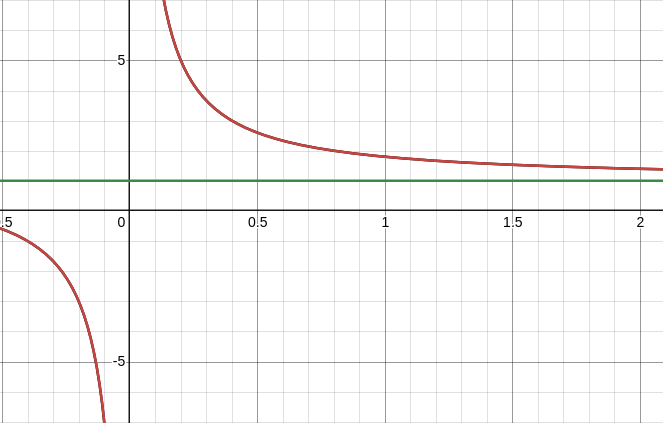
\includegraphics[width=0.7\textwidth]{figures/IMG_ch7/FR/FRH0} % Adjust the width as needed
    \caption{$\lambda$ = 0.8 $\theta$ = 0.  x-axis: $\delta$. With smaller delta, there is an increasingly large burst size.  In this plot the removal value, $\theta$ is 0. On the y-axis is the quantity $ \mean{\text{max}(0, r-\theta)} $  and $\mean{r}$, the mean release without removal. When $\theta = 0$, these two values are obviously the same, and the lines overlap. In the figures below,  $\theta  \neq 0$,  and the lines do not overlap.}
    \label{fig:sinfigure}
\end{figure}



\begin{figure}[H]
    \centering
    % First figure
    \begin{subfigure}{0.48\textwidth}
        \centering
        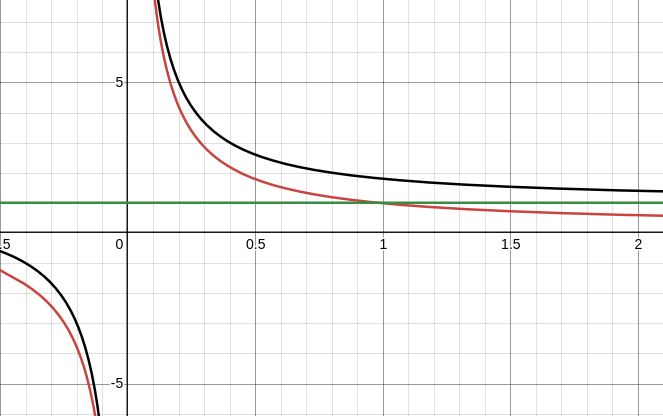
\includegraphics[width=\textwidth]{figures/IMG_ch7/FR/FRH0p8} % Adjust the image path as necessary
    \end{subfigure}
    \hspace{\fill} % Optional: adds space between figures
    % Second figure
    \begin{subfigure}{0.48\textwidth}
        \centering
        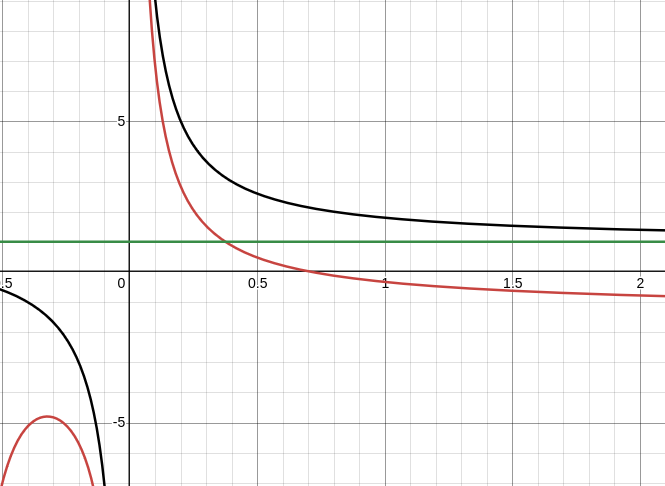
\includegraphics[width=\textwidth]{figures/IMG_ch7/FR/FRH2p3_L0p8} % Adjust the image path as necessary
    \end{subfigure}
    
    \caption{It can be seen that when $\theta > 0$, the required $\delta$ to ensure supercritical proliferation ($\mean{\text{max}(0, r-\theta)} > 1$) is smaller (the required release size is higher). ( $\lambda$ = 0.8, $\theta$ = 0.8 and $\theta = 2.3$ (left and right respectively))}
    \label{}
\end{figure}



\subsubsection{Motivation}

I am interested in the question of whether there is some fundamental advantage to bursting dynamics in pathogenesis. In the case of \ft \, and \yp, hot cell lysis may be caused merely as the simplest means of release. With bacteria being relatively large in comparison to the protein complexes that constitute a cell membrane, it would be difficult to employ a strategy in which some but not all of the pathogen are released. The case of viruses is different. They are sufficiently small to allow for partial release of an intracellular load. To be fair, in the case of viruses such as HIV, there is an explicit advantage to not killing the cell: its machinery continues to produce virions. Despite this, I have a suspicion that there is some advantage to bursting style strategies. That is, where agents are released in large groups all at once from their hidden position within host cells. As opposed to continually, or in dribs and drabs. There are a great many stories one could tell about the reason for which this might be the case, that there is an advantage to bursting. Here are three categories in which the ones I've thought up fall under. 

\begin{itemize}
\item \textbf{Subductive proliferation.} Replication rate reduces over time within a host cell, perhaps following recognition, or by the using up of available resources. (Though to be honest, I'm starting to think that this doesn't check out as a reason --- some analysis should reveal the truth one way or the other).
\item  \textbf{Limited extracellular killing.} As described above, the means of removing agents are finite on relevant timescales, this leading to an effective reduction in death rate for invading pathogen. Note: this dynamic my take place either inside the cell or extracellularly as described above. For the case of within cell dynamics, some host cells contain oxidative granules, which in their finite number, destroy intracellular agents.  
\item \textbf{Detection avoidance}
For the case of HIV, where observations have been made that release is sporadic and clustered. There may be some argument against a strategy of continual budding because it might lead to more effective detection by targeting immune cells which induce apoptosis. 
\end{itemize}
Each argument of these three types essentially boils down to the catching off guard of some immune mechanism. As it were, surprising the systems of regulation to the extent that response is too slow. 



\subsubsection{Potential for \yp}

We might be able to frame this model in the context of Y. pestis and neutrophils. That is, the target cells are macrophages, the killer cells are neutrophils. And the reason for the two phases of infection is argued for by firstly, the advantage of bursting in the case of constant density killer cells, then secondly, the mass increase in killer cells causes a need to become extracellular. But this would beg the question: why not just replicate extracellularly from the beginning. There must be some advantage to being within macrophages. For one thing, they are a means of transport. Taking the agents to lymph nodes where there is lots of food. They may provide food themselves.
